\documentclass[11pt]{beamer}
\usetheme{Copenhagen}
\usecolortheme{dolphin}
\usepackage{epsfig}
\usepackage{amsmath}
\usepackage{tabu}
\usepackage{amsfonts}
\usepackage{latexsym}
\usepackage[utf8]{inputenc}
\usepackage{listings}    
\usepackage[catalan]{babel}
\usepackage{newunicodechar}
\usepackage{graphicx}
\usepackage{subcaption}
\usepackage{float}
\usepackage{pgf, tikz}
\usepackage{listings}

\setcounter{tocdepth}{4}
\setcounter{secnumdepth}{4}

\newunicodechar{Ŀ}{\L.}
\newunicodechar{ŀ}{\l.}

\definecolor{dkgreen}{rgb}{0,0.6,0}
\definecolor{gray}{rgb}{0.5,0.5,0.5}
\definecolor{mauve}{rgb}{0.58,0,0.82}

\geometry{paperwidth=150mm,paperheight=115mm}

\usepackage{hyperref}
\hypersetup{
  colorlinks=false, %set true if you want colored links
  linktoc=all,     %set to all if you want both sections and subsections linked
  linkcolor=blue,  %choose some color if you want links to stand out
}

\title[Generació d'horaris d'institut amb operacions lògiques]{GENERACIÓ D'HORARIS D'INSTITUT AMB OPERACIONS LÒGIQUES}
\author{Ismael El Habri \\ \footnotesize Tutors: Dr. Josep Suy i Dr. Jordi Coll}
\institute{Universitat de Girona}

\date[KPT 2004] % (optional)
{10 de setembre del 2019}

\AtBeginSection[]
{
  \begin{frame}
    \frametitle{Table of Contents}
    \tableofcontents[currentsection]
  \end{frame}
}
\begin{document}

\frame{\titlepage}

\section{Introducció}
  \begin{frame}
    \frametitle{Introducció}

    Confecció d'horaris, problema recurrent amb el que es troben els instituts $\Rightarrow$ High School TimeTabling problem (HSTT)\\ ~\\
    
    \begin{itemize}
      \item Alta combinatòria i complexitat, és un problema NP-Complet.
      \item Repartir events i recursos de manera viable i tenint en compte preferències del professorat.
      \item Diferents països, diferents necessitats  $\Rightarrow$  més complexitat!
    \end{itemize}
    
    


  \end{frame}
  \subsection{Marc de treball}
  \begin{frame}
    \frametitle{Marc de treball}
    \begin{itemize}
      \item Grup de recerca de Lògica i Programació
    
      \item API SMT desenvolupada pel Dr. Jordi Coll. API per a la codificació de problemes SAT, SMT o MaxSAT, 
      actuant com a interfície per a diferents solvers. En aquest treball s'utilitzarà el Yices 2. 
      També té implementades les diferents implementacions de múltiples restriccions globals.

      \item Com a punt de partida s'ha utilitzat el treball realitzat el 2015 per en Cristòfor Nogueira. 
      Mentre ell ha utilitzat BitVectors i MaxSAT, en aquest treball s'utilitzarà SMT. 
      Així s'han aconseguit uns resultats superiors pel que fa el temps d'execució.
    \end{itemize}

  \end{frame}
  
  \subsection{Objectius}

  \begin{frame}
    \frametitle{Objectius}

    \begin{itemize}
    
      \item Aprofundir sobre el tema.
       \begin{itemize}
        \item Problema de generació d'horaris d'institut.
        \item Problemes de satisfacció de restriccions(CSP).
        \item Tècniques per resoldre problemes CSP com ara SAT i extensions.
       \end{itemize}
      \item Crear un generador.
    
    \end{itemize}
          
  \end{frame}
  
  \subsection{Metodologia}
  \begin{frame}
    \frametitle{Metodologia}
    \begin{itemize}
      \item Estudi del treball prèvi i estat de l'art
      \item Entregues periòdiques
      \item Prototipatge
    \end{itemize}

  \end{frame}

  \begin{frame}
    \frametitle{Estudi de viabilitat}

  \end{frame}

  \section{Implementació}
  
  \begin{frame}
  \frametitle{Implementació}
    \begin{figure}[p]
      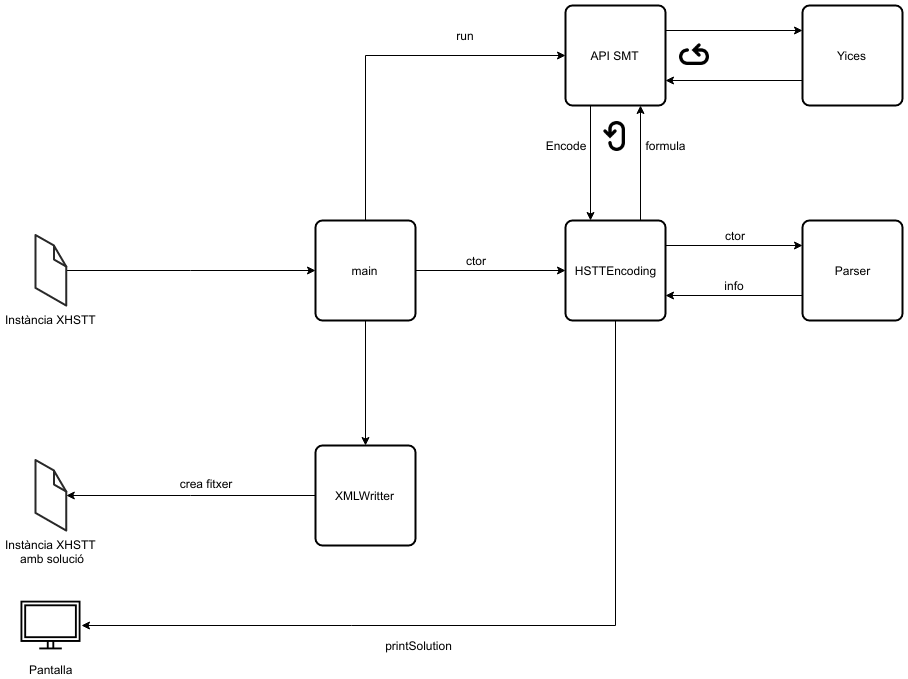
\includegraphics[width=\textwidth]{Diagrames/Arqui2.png}
      \label{fig:procs}
    \end{figure}
  \end{frame}

  
  \subsection{Parser}
  
  \begin{frame}
    \frametitle{Parser}

    Instància XHSTT $\Rightarrow$ dades + restriccions


  \end{frame}

  \subsection{Model}
  
  \begin{frame}
    \frametitle{Model}

    \begin{itemize}
      \item $Xt_{0,0} . . . Xt_{|Events|-1,|Times|-1}$
      \item $Xs_{0,0} . . . Xs_{|Events|-1,|Times|-1}$
      \item $Xd_{0,1,0} . . . Xd_{|Events|-1, event.duration, |Times|-1}$
    \end{itemize}
  \end{frame}

  \begin{frame}
  \frametitle{Clàusules de Channeling}  

  \begin{itemize}
    \item Si un event comença a una hora determinada, llavors té una duració: \begin{center} $\forall e \in 0 ... |Events|-1$ $\forall i \in 0 ... |Times|-1$ \\$exactly\_one(\neg Xs_{e,i} \vee \{ \forall j \in 1 ... e.duration$ $Xd_{e,j,i}\})$\end{center}
    \item Si un event té lloc a t però no a t-1, és que comença: \begin{center} $\forall e \in 0 ... |Events|-1$ $\forall i \in 0 ... |Times|-1$ \\$\neg Xt_{e,i} \vee Xt_{i-1} \vee Xs_i$ \end{center}
    \item Si un event comença amb duració d, llavors té lloc en d hores consecutives: \begin{center} 
      $\forall e \in 0 ... |Events|-1$ $\forall d in 1 ... e.duration$ $\forall i \in 0 ... |Times|-1$ $\forall j \in i ... i+d-1$ \\
      $\neg Xd_{e,d,i} \vee Xt_{e,j}$    
    \end{center}
  \end{itemize}

  \end{frame}

  \subsection{Restriccions}

  
  \begin{frame}
    \frametitle{Restriccions}

    \begin{itemize}
      \item Assign Times Constraint \[
        \forall e \in Events \ exactly_k(\{Xt_{e,0} ... Xt_{e,|Times|-1}\}, e.duration)
      \]
      \item Split Events Constraint
      \begin{gather*}
        \forall e \in Events \ at\_most\_k(\{Xs_{e,0} . . . Xs_{e,|Times|-1}\}, MaximumAmount)\\
        \forall e \in Events \ at\_least\_k(\{Xs_{e,0} . . . Xs_{e,|Times|-1}\}, MinimumAmount)\\
        \forall e \in Events \ \forall d \notin MinimumDuration...MaximumDuration \land d \in 1 ... e.duration  \\
        \forall t \in 0...|Times|-1 \quad \neg Xd_{e,d,t}
      \end{gather*}
      \item Distribute Split Constraint
      \begin{gather*}
      \forall e \in Events \ at\_most\_k(\{Xd_{e,d,0} .... Xd_{e,d,|Times|-1}\}, max) \quad \quad si \ max<\frac{e.duration}{d}\\
      \forall e \in Events \ at\_most_k(\{Xd_{e,d,0} .... Xd_{e,d,|Times|-1}\}, min) \quad \quad \quad si \ min>0\\
      \end{gather*}
    \end{itemize}
  
  \end{frame} 
  \begin{frame}
    \frametitle{Restriccions}

    \begin{itemize}

      \item Prefer Times Constraint
      \begin{gather*}
        \forall e \in Events \ \forall t \in Times \land t \notin Ta \\ (\neg Xd_{e,d,t})
      \end{gather*}
      \item Spread Events Constraint
        \begin{align*}
          \forall e \in Events \ &\forall g \in Tg \\
          &at\_most\_k(\{Xs_{e,t} | t \leftarrow g\}, max)\\
          \forall e \in Events \ &\forall g \in Tg \\
          &at\_least\_k(\{Xs_{e,t} | t \leftarrow g\}, max)
        \end{align*}    
      \item Avoid Clashes Constraint
        \begin{align*}
          \forall r \in Resources \ & \forall t \in Times \\
          &at\_most\_one(\{Xt_{e,t} | e \leftarrow E_r\})
        \end{align*}

        \item Avoid Unavailable Times Constraint
        \begin{align*}
          \forall r \in Resources \ \forall t \in T \ \forall e \in E_r \quad
          (\neg Xt_{e,t})
        \end{align*}
    
    \end{itemize}
  
  \end{frame}
  \begin{frame}
    \frametitle{Restriccions}

    \begin{itemize}
      \item Limit Idle Times Constraint

      Per a cada recurs $r$ es fan les clàusules següents:

       \begin{align*}
        \forall g \in Tg \ \forall t \in g \ &\forall e \in E_r \\
        &(\neg Idle_i \lor \neg Xt_{e, t}) & si \ \ (B_t \neq \emptyset \ \& A_t \neq \emptyset) \\
        \forall g \in Tg \ \forall t \in g  \ & \\
        & (\neg Idle_t \lor \{\forall b \in B_t \ \forall e \in E_r \ Xt_{e,b}\}) & si \ \ (B_t \neq \emptyset)\\
        \forall g \in Tg \ \forall t \in g & \\
        & (\neg Idle_t \lor \{\forall a \in A_t \ \forall e \in E_r \ Xt_{e,a}\}) & si \ \ (A_t \neq \emptyset)\\
        \forall g \in Tg \ \forall t \in g \ \forall b \in B_t \ \forall a \in A_t & \\
        \forall e1 \in E_r \ \forall e_2 \in E_r \ \forall e_3 \in E_r & \\
        & (Xt_{e_{1}, t} \lor \neg Xt_{e_2, b} \lor Xt_{e_3, a} \lor Idle_t) & si \ \ (B_t \neq \emptyset \ \& A_t \neq \emptyset)
       \end{align*}
    
       Un cop definides i lligades les variables auxiliars l'únic que queda és, per cada recurs, imposar les restriccions de cardinalitat:
    
       \begin{align*}
        \forall r \in Resources &\\
        & at\_most\_k(\{ Idle_t | t \leftarrow Times\}, max) \\
        & at\_least\_k(\{ Idle_t | t \leftarrow Times\}, min)
       \end{align*}
    \end{itemize}
  
  \end{frame}
  \begin{frame}
    \frametitle{Restriccions}

    \begin{itemize}
    
      \item Cluster Busy Times Constraint \\
      Per a cada recurs $r$ es fan les clàusules següents:
      
      \begin{align*}
        \forall g \in Tg & \\
        &(\neg Busy_g \lor (\forall e \in E_r \ \forall t \in g \quad Xt_{e,t}))\\
        \forall g \in Tg \ \forall t \in g \ \forall e \in E_r &\\
        & (\neg Xt_{e,t} \lor Bsuy_g)
      \end{align*}
    
      Un cop definides i lligades les variables auxiliars l'únic que queda és, per cada recurs, imposar les restriccions de cardinalitat:
      \begin{align*}
        \forall r \in Resources &\\
        & at\_most\_k(\{ Busy_g | g \leftarrow Tg\}, max) \\
        & at\_least\_k(\{ Busy_g | g \leftarrow Tg\}, min)
       \end{align*}
          
    \end{itemize}
  
  \end{frame}


  \section{Conclusions i Resultats}
  \subsection{Resultats}
  
  \begin{frame}
    \frametitle{Resultats resolució}
    \begin{itemize}
      \item 
    \end{itemize}

  \end{frame}

  \begin{frame}
    \frametitle{Resultats optimització}
  \end{frame}

  \subsection{Conclusions}

  
  \begin{frame}
  \end{frame}




  
\end{document}